\documentclass[11pt]{amsart}
\usepackage[margin=1.1in]{geometry}
\usepackage{amssymb,booktabs,hyperref,tikz}
\hypersetup{colorlinks=true,linkcolor=blue,citecolor=blue,urlcolor=blue}

\newtheorem{theorem}{Theorem}[section]
\newtheorem{proposition}[theorem]{Proposition}
\newtheorem{lemma}[theorem]{Lemma}
\newtheorem{corollary}[theorem]{Corollary}
\newtheorem{conjecture}[theorem]{Conjecture}
\theoremstyle{definition}
\newtheorem{definition}[theorem]{Definition}
\newtheorem{remark}[theorem]{Remark}

\newcommand{\tr}{\operatorname{tr}}
\newcommand{\Q}{\mathbb{Q}}
\newcommand{\Z}{\mathbb{Z}}

\title[Double eigenvalues of Fibonacci-weighted cycles]{Double eigenvalues of cycles weighted by the Fibonacci word}
\author{Vamshi Jandhyala}
\date{Preprint, version 1, 21 November 2026. Not peer reviewed. Zenodo: \href{https://doi.org/10.5281/zenodo.24419102}{doi:10.5281/zenodo.24419102}.}
\subjclass[2020]{05C50, 15A18, 68R15, 47B36}
\keywords{weighted cycle, Laplacian spectrum, Fibonacci word, transfer matrix, trace map, $2$-adic valuation}

\begin{document}

\begin{abstract}
Give the edges of the $n$-cycle the weights $a$ and $b$ in the order of the letters of the Fibonacci word
$ABAABABAAB\cdots$. Foltz observed (OEIS A401899, weights $1$ and $2$) that the Laplacian has only $3F_k$
distinct eigenvalues when $n=4F_k$, and that every other $n\le 400$ has $n$ distinct eigenvalues except for
a sparse set where one eigenvalue is double. We prove the first statement for all $k\ge4$ and all positive
weights $a\ne b$: the $4F_k$-cycle has exactly $F_k$ double eigenvalues, namely the spectrum of the
$F_k$-cycle twisted by the phase $i$, and all its other eigenvalues are simple. For the weights $1$ and $2$
we show that $1$ is a double eigenvalue of the $n$-cycle exactly when $n\in\{20,33,53,106\}$, so the sparse
set is finite at that eigenvalue. The proof of the second result is $2$-adic. An exact computation for
$n\le 6000$ finds no other double eigenvalues, and none at all off $n=4F_k$ for four other pairs of weights.
\end{abstract}

\maketitle

\noindent\emph{Status of this preprint.} Every count and exceptional set quoted is computed exactly over $\Q$
by the programs described in \emph{Code and data} (decimal eigenvalues are rounded, and one independent recheck is
numerical); each of these programs asserts its results and exits with an error on
failure, and planted wrong inputs are rejected. There is no formal (Lean) verification. This version has not yet been independently
reviewed.

\section{Introduction}

Let $f=f_1f_2f_3\cdots=ABAABABAABAAB\cdots$ be the Fibonacci word, the fixed point of the substitution
$A\mapsto AB$, $B\mapsto A$. Fix positive reals $a\ne b$ and let $C_n$ be the weighted cycle on vertices
$1,\dots,n$ whose edge $\{i,i+1\}$ (indices mod $n$) has weight $w_i=a$ if $f_i=A$ and $w_i=b$ if $f_i=B$.
Its Laplacian $L_n$ acts by
\[
(L_nx)_i=w_{i-1}(x_i-x_{i-1})+w_i(x_i-x_{i+1}).
\]
Write $d(n)=n-\#\{\text{distinct eigenvalues of }L_n\}$ for the \emph{deficit}. For $a=1$, $b=2$ the number of
distinct eigenvalues is OEIS A401899, contributed by Scott M.~Foltz on 15 November 2026 \cite{OEIS}. Its
comment records that for $n\le400$ the deficit is positive only at
$n=12,20,32,33,52,53,84,106,136,220,356$, with values $3,5,8,1,13,1,21,1,34,55,89$, and conjectures that
$d(4F_k)=F_k$ for $k\ge4$ and that otherwise $d(n)=0$ except on a sparse set with deficit $1$.
Here $F_1=F_2=1$.

\begin{theorem}\label{thm:main}
Let $a,b>0$, $a\ne b$, and $k\ge4$. Then $L_{4F_k}$ has exactly $F_k$ double eigenvalues and all its other
eigenvalues are simple; so $d(4F_k)=F_k$. The double eigenvalues are the eigenvalues of the $F_k$-cycle on the
first $F_k$ letters of $f$ with the edge $\{F_k,1\}$ twisted by the phase $i$.
\end{theorem}

\begin{theorem}\label{thm:one}
Let $a=1$, $b=2$. The number $1$ is a double eigenvalue of $L_n$ if and only if $n\in\{20,33,53,106\}$.
\end{theorem}

The smallest case shows the mechanism. For $n=12$ the word is $ABAABABAABAA$, and it reads $U\,U\,V\,V$ with
$U=ABA$ and $V=BAA$, a rotation of $U$ (Figure~\ref{fig:cycle}). With weights $1$ and $2$ the three double
eigenvalues of $L_{12}$ are approximately $0.3187$, $2.3579$ and $5.3234$, the roots of $\lambda^3-8\lambda^2+15\lambda-4$, which
is $-2$ times the trace of the transfer matrix of the three-letter block $ABA$ (Section~2). A block whose transfer
matrix has trace zero squares to $-I$; two such squares in a row return to $I$, and that makes the eigenvalue double.

\begin{figure}[ht]
\centering
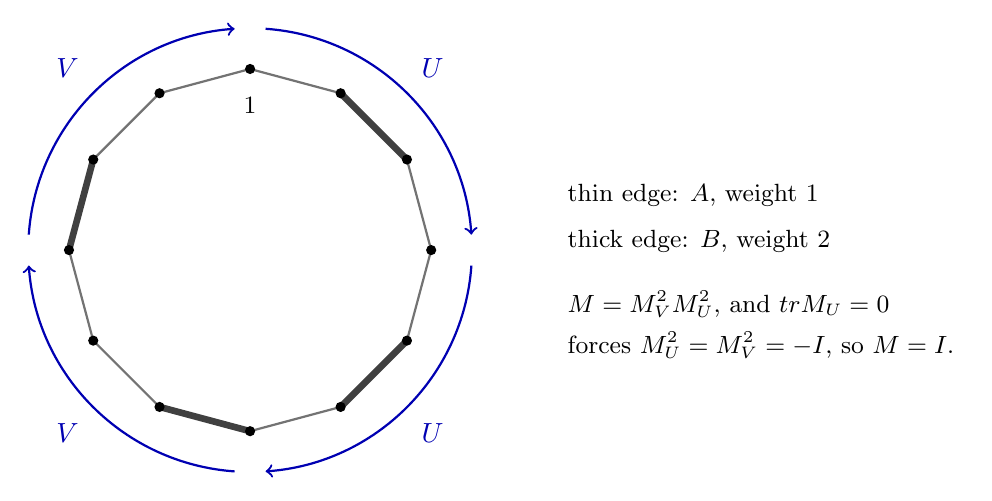
\begin{tikzpicture}[scale=1.15]
  \def\w{{1,2,1,1,2,1,2,1,1,2,1,1}}
  \foreach \i in {0,...,11} {
    \pgfmathsetmacro{\a}{90-30*\i}\pgfmathsetmacro{\b}{90-30*(\i+1)}
    \pgfmathsetmacro{\ww}{\w[\i]}
    \ifdim\ww pt>1pt \draw[line width=2.4pt,black!75] (\a:2) -- (\b:2);
    \else \draw[line width=0.8pt,black!55] (\a:2) -- (\b:2); \fi
  }
  \foreach \i in {0,...,11} \fill (90-30*\i:2) circle (1.6pt);
  \foreach \lab/\s in {U/0,U/3,V/6,V/9} {
    \draw[blue!70!black,thick,->] ({90-30*\s-4}:2.45) arc ({90-30*\s-4}:{90-30*(\s+3)+4}:2.45);
    \node[blue!70!black] at ({90-30*(\s+1.5)}:2.85) {$\lab$};
  }
  \node at (90:1.6) {\small $1$};
  \node[align=left,anchor=west] at (3.4,0.6) {\small thin edge: $A$, weight $1$};
  \node[align=left,anchor=west] at (3.4,0.1) {\small thick edge: $B$, weight $2$};
  \node[align=left,anchor=west] at (3.4,-0.6) {\small $M=M_V^2M_U^2$, and $\operatorname{tr}M_U=0$};
  \node[align=left,anchor=west] at (3.4,-1.05) {\small forces $M_U^2=M_V^2=-I$, so $M=I$.};
\end{tikzpicture}
\caption{The $12$-cycle on $ABAABABAABAA$, starting at vertex $1$ and going clockwise. The word is $UUVV$ with
$U=ABA$ and $V=BAA$ (Lemma~\ref{lem:word}). Going once round multiplies the transfer matrices of the four blocks.
At each of the three roots of $\operatorname{tr}M_U=0$ the product is $I$, so the eigenvalue is double
(Lemmas~\ref{lem:fixed} and~\ref{lem:three}).}
\label{fig:cycle}
\end{figure}

So the three sporadic values $33,53,106$ of the OEIS comment are the only ones at the eigenvalue $1$, and
$n=20$ belongs to Theorem~\ref{thm:main}. We also show $d(F_k)=d(2F_k)=0$ for every $a\ne b$
(Proposition~\ref{prop:easy}). Section~\ref{sec:comp} reports an exact search: for $a=1$, $b=2$ and
$n\le6000$ the only double eigenvalues off $n=4F_k$ are the three of Theorem~\ref{thm:one}, and for four other
pairs of weights there are none off $n=4F_k$ for $n\le2000$. This supports Conjecture~\ref{conj}.

The tools are standard in the study of the Fibonacci Hamiltonian: transfer matrices, the trace map of
Kohmoto, Kadanoff and Tang \cite{KKT}, and its invariant. The observation that a transfer block of trace
zero squares to $-I$ is used by Chattopadhyay and Chakrabarti \cite{CC} to explain cycles of the matrix map
of Fibonacci chains; see also \cite{KST}. What is new here is the exact count: the factorisation of the
prefix of length $4F_k$ (Lemma~\ref{lem:word}), a reduction of the double-eigenvalue condition to three cases
(Lemma~\ref{lem:three}), the exclusion of two of them for all weights, and the $2$-adic argument behind
Theorem~\ref{thm:one}.

\section{Transfer matrices}

For $w>0$ and a real parameter $\lambda$ put
\[
E(w)=\begin{pmatrix}1&1/w\\0&1\end{pmatrix},\qquad S=\begin{pmatrix}1&0\\-\lambda&1\end{pmatrix},\qquad
T(w)=E(w)S,
\]
all of determinant $1$. Let $y_i=w_i(x_{i+1}-x_i)$ be the flux through edge $i$. The eigenvalue equation
$\lambda x_i=(L_nx)_i$ reads $\lambda x_i=y_{i-1}-y_i$, so
\[
\begin{pmatrix}x_{i+1}\\y_i\end{pmatrix}=T(w_i)\begin{pmatrix}x_i\\y_{i-1}\end{pmatrix}.
\]
For a word $u=u_1\cdots u_m$ over $\{A,B\}$ let $M_u=T(w(u_m))\cdots T(w(u_1))$, where $w(A)=a$, $w(B)=b$, so
that $M_{uv}=M_vM_u$. Let $M^{(n)}$ be $M_u$ for $u=f_1\cdots f_n$.

\begin{lemma}\label{lem:fixed}
The $\lambda$-eigenspace of $L_n$ is isomorphic to the space of fixed vectors of $M^{(n)}(\lambda)$. Hence
every eigenvalue has multiplicity at most $2$, $\lambda$ is double exactly when $M^{(n)}(\lambda)=I$, and
$d(n)=\#\{\lambda\in\mathbb{R}:M^{(n)}(\lambda)=I\}$.
\end{lemma}

\begin{proof}
An eigenvector $x$ gives $(x_1,y_0)$ with $y_0=y_n$, which $M^{(n)}$ fixes. Conversely a fixed vector
$(x_1,y_0)$ generates by the recursion a sequence with $x_{n+1}=x_1$ and $y_n=y_0$, which is an eigenvector.
Both maps are linear and inverse to each other.
\end{proof}

For a word $u$ of length $N$ the entry polynomials of $M_u$ have degree at most $N$, and $\tr M_u$ has
degree exactly $N$ with leading coefficient $(-1)^N/\prod w(u_i)$: the coefficient of $\lambda$ in $T(w)$ is
$\left(\begin{smallmatrix}-1/w&0\\-1&0\end{smallmatrix}\right)$, and the product of these matrices has
top-left entry $\prod(-1/w(u_i))$.

\begin{lemma}\label{lem:twist}
Let $u$ have length $N$ and $\theta\in(0,\pi)$. Then $\tr M_u(\lambda)=2\cos\theta$ has exactly $N$ real
roots, all simple. They are the eigenvalues of the cycle on $u$ with the edge $\{N,1\}$ twisted by
$e^{i\theta}$.
\end{lemma}

\begin{proof}
The twisted cycle has a Hermitian Laplacian $L^\theta$: in the formula for $L_n$, replace $x_{N+1}$ by
$e^{i\theta}x_1$ and $x_0$ by $e^{-i\theta}x_N$. As in Lemma~\ref{lem:fixed}, $\lambda$ is an eigenvalue of
$L^\theta$ exactly when $M_u(\lambda)$ has eigenvalue $e^{i\theta}$, with multiplicity equal to the dimension
of that eigenspace. Since $\det M_u=1$, this happens exactly when $\tr M_u(\lambda)=2\cos\theta$, and then the
eigenvalues $e^{\pm i\theta}$ are distinct, so the eigenspace is a line. Thus $L^\theta$ has $N$ distinct real
eigenvalues, each a root of the degree-$N$ polynomial $\tr M_u-2\cos\theta$.
\end{proof}

This is the discrete Floquet theory of periodic Jacobi matrices; see \cite[Section~7.2]{Teschl}.

\section{The Fibonacci word}

Put $s_0=B$, $s_1=A$ and $s_{j+1}=s_js_{j-1}$, so $s_j=\varphi^{j-1}(A)$ for $j\ge1$, where $\varphi$ is the
substitution, and $|s_j|=F_{j+1}$. For $j\ge1$ the word $f$ begins with $s_j$.

\begin{lemma}\label{lem:word}
Let $m\ge3$, $U=s_m$, $x=s_{m-2}$ and $y=s_{m-3}s_{m-2}$. Then $U=xy$, and the first $4|U|$ letters of $f$ are
$UUVV$ with $V=yx$.
\end{lemma}

\begin{proof}
From $s_m=s_{m-1}s_{m-2}=s_{m-2}s_{m-3}s_{m-2}$ we get $U=xy$. Using $s_{m-2}s_{m-3}=s_{m-1}$,
\begin{align*}
UUVV&=s_m\,s_{m-1}s_{m-2}\,s_{m-3}s_{m-2}s_{m-2}\,s_{m-3}s_{m-2}s_{m-2}\\
&=s_m\,s_{m-1}\,s_{m-1}s_{m-2}\,s_{m-1}s_{m-2}\,s_{m-2}.
\end{align*}
On the other hand $f$ begins with
\[
s_{m+3}=s_{m+2}s_{m+1}=s_ms_{m-1}s_ms_ms_{m-1}=s_m\,s_{m-1}\,s_{m-1}s_{m-2}\,s_{m-1}s_{m-2}\,s_{m-1}.
\]
The two words agree up to the last block, and the
first $|s_{m-2}|$ letters of $s_{m-1}=s_{m-2}s_{m-3}$ are $s_{m-2}$.
\end{proof}

Write $x_j=\tr M_{s_j}$ for $j\ge0$, and define $M_{s_{-1}}=M_AM_B^{-1}$ (so that formally $s_1=s_0s_{-1}$)
and $x_{-1}=\tr M_{s_{-1}}$. For $2\times2$ matrices of determinant $1$ we use
$\tr(XY)=\tr X\tr Y-\tr(XY^{-1})$ and Fricke's identity
$\tr[X,Y]=(\tr X)^2+(\tr Y)^2+(\tr XY)^2-\tr X\tr Y\tr XY-2$, where $[X,Y]=XYX^{-1}Y^{-1}$.

\begin{lemma}[trace map \cite{KKT}]\label{lem:trace}
For $j\ge1$, $x_{j+1}=x_jx_{j-1}-x_{j-2}$, and $\tr[M_{s_j},M_{s_{j-1}}]=\tr[M_A,M_B]$ for $j\ge1$. Moreover
\[
\tr[M_A,M_B]-2=\frac{\lambda^2(a-b)^2}{a^2b^2},\qquad x_{-1}=2,
\]
\[
x_0=2-\frac{\lambda}{b},\qquad x_1=2-\frac{\lambda}{a},\qquad x_2=\frac{\lambda^2-2(a+b)\lambda+2ab}{ab}.
\]
\end{lemma}

\begin{proof}
$M_{s_{j+1}}=M_{s_{j-1}}M_{s_j}$ and $M_{s_{j-1}}M_{s_j}^{-1}=M_{s_{j-2}}^{-1}$ (from
$M_{s_j}=M_{s_{j-2}}M_{s_{j-1}}$), which gives the recursion. The pair $(M_{s_{j+1}},M_{s_j})=(YX,X)$ for
$(X,Y)=(M_{s_j},M_{s_{j-1}})$, and $[YX,X]=YXY^{-1}X^{-1}=[Y,X]=[X,Y]^{-1}$ has the same trace. The four
values are direct computations; $M_{s_{-1}}=E(a)E(b)^{-1}=E(ab/(b-a))$ is unipotent.
\end{proof}

\section{Proof of Theorem~\ref{thm:main}}

The plan has three steps. By Lemma~\ref{lem:word} the transfer matrix of the $4F_k$-cycle is $M_V^2M_U^2$ with $V$ a
rotation of $U$, so $M_U$ and $M_V$ are conjugate. A $2\times2$ identity (Lemma~\ref{lem:three}) shows that this
product is $I$ in only three situations: $\tr M_U=0$, two traces vanishing together, or $M_U=\pm I$. The first
gives exactly $F_k$ double eigenvalues by Lemma~\ref{lem:twist}. The other two cannot happen when $a\ne b$: $M_U=\pm I$ is
ruled out by the invariant of the trace map (Lemma~\ref{lem:noiii}), and two consecutive vanishing traces by running
the trace recursion down to its initial values (Lemma~\ref{lem:noii}).

\begin{lemma}\label{lem:three}
Let $m\ge3$ and $U,V,x,y$ be as in Lemma~\ref{lem:word}. Then $M^{(4|U|)}(\lambda)=I$ if and only if one of
the following holds: (i) $\tr M_U=0$; (ii) $\tr M_x=\tr M_y=0$; (iii) $M_U=\pm I$.
\end{lemma}

\begin{proof}
Put $P=M_x$, $Q=M_y$, $C=M_U=QP$ and $D=M_V=PQ$; both have trace $t$. By Lemma~\ref{lem:word},
$M^{(4|U|)}=D^2C^2$. By Cayley--Hamilton $D^2=tD-I$ and $C^{-2}=tC^{-1}-I$, so $D^2C^2=I$ if and only if
$t(D-C^{-1})=0$, that is, $t=0$ or $PQQP=I$. With $p=\tr P$, $q=\tr Q$, the second condition $Q^2=P^{-2}$
reads $qQ=pP^{-1}$. If $p=q=0$ this holds. If exactly one of $p,q$ is $0$ it fails, since $P,Q$ are
invertible. Otherwise $Q=(p/q)P^{-1}$, and taking determinants $p/q=\pm1$, so $C=QP=\pm I$. Conversely each
of (i), (ii), (iii) gives $D^2C^2=I$: in (i) $C^2=D^2=-I$; in (ii) $P^2=Q^2=-I$; in (iii) $D=PCP^{-1}=C$.
\end{proof}

\begin{lemma}\label{lem:noiii}
For every $j\ge2$ and real $\lambda$, $M_{s_j}(\lambda)\ne\pm I$.
\end{lemma}

\begin{proof}
If $M_{s_j}=M_{s_{j-2}}M_{s_{j-1}}=\pm I$ then $M_{s_{j-1}}$ and $M_{s_{j-2}}$ commute, so their commutator has
trace $2$, and by Lemma~\ref{lem:trace} $\lambda^2(a-b)^2=0$, so $\lambda=0$. At $\lambda=0$ every $T(w)$ equals $E(w)$, so
$M_{s_j}(0)$ is upper unitriangular with upper-right entry $\sum_i 1/w(u_i)>0$, the sum over the letters of
$s_j$; it is not $\pm I$.
\end{proof}

\begin{lemma}\label{lem:noii}
For every $j\ge2$ and real $\lambda$, $x_j$ and $x_{j-1}$ do not vanish together.
\end{lemma}

\begin{proof}
Suppose $x_j=x_{j-1}=0$ with $j\ge3$. The recursion at $j$ gives $x_{j-3}=0$ and at $j-1$ gives $x_{j-4}=0$.
Descending by $3$ we reach a common zero of $(x_2,x_1)$, $(x_1,x_0)$ or $(x_0,x_{-1})$. But $x_{-1}=2$;
$x_1=0$ only at $\lambda=2a$ and $x_0=0$ only at $\lambda=2b\ne2a$; and $x_2(2a)=-2$.
\end{proof}

\begin{proof}[Proof of Theorem~\ref{thm:main}]
Let $m=k-1\ge3$, so $|U|=|s_m|=F_k$. By Lemma~\ref{lem:fixed}, $d(4F_k)$ counts the $\lambda$ with
$M^{(4F_k)}(\lambda)=I$. Case (iii) of Lemma~\ref{lem:three} never occurs, by Lemma~\ref{lem:noiii}. In case
(ii), $\tr M_x=x_{m-2}$, and $\tr M_y=x_{m-1}$ because $y=s_{m-3}s_{m-2}$ is a rotation of
$s_{m-1}=s_{m-2}s_{m-3}$; so case (ii) never occurs, by Lemma~\ref{lem:noii} with $j=m-1\ge2$. Case (i) holds
at exactly $F_k$ real values of $\lambda$, by Lemma~\ref{lem:twist} with $\theta=\pi/2$, and these are the
eigenvalues of the twisted cycle.
\end{proof}

\begin{proposition}\label{prop:easy}
For $a,b>0$, $a\ne b$ and $k\ge4$: $d(F_k)=0$ and $d(2F_k)=0$.
\end{proposition}

\begin{proof}
$M^{(F_k)}=M_{s_{k-1}}\ne I$ by Lemma~\ref{lem:noiii}. By Lemma~\ref{lem:word} the first $2F_k$ letters are
$UU$, so $M^{(2F_k)}=M_U^2$; if this is $I$ then $M_U=\pm I$, again excluded.
\end{proof}

\section{The eigenvalue $1$ for weights $1$ and $2$}

Take $a=1$, $b=2$, $\lambda=1$. Then $M_A=\left(\begin{smallmatrix}0&1\\-1&1\end{smallmatrix}\right)$ and
$M_B=\left(\begin{smallmatrix}1/2&1/2\\-1&1\end{smallmatrix}\right)$ lie in $SL_2(\Z[1/2])$. Put
$P_j=M_{s_j}(1)$. Let $v_2$ be the $2$-adic valuation on $\Q$, and for a matrix $X$ over $\Q$ let
$\ell(X)=-\min v_2(X_{rs})$ over its entries, so that $2^{\ell(X)}$ is the $2$-adic max norm. Then
$\ell(XY)\le\ell(X)+\ell(Y)$ and, for $\det X=1$, $\ell(X^{-1})=\ell(X)$. Put $\ell_j=\ell(P_j)$.

\begin{lemma}\label{lem:escape}
$v_2(x_j(1))=-F_{j-7}$ for $j\ge9$, and $\ell_j=F_{j-7}$ for $j\ge7$; also $\ell_j\le1$ for $0\le j\le8$.
\end{lemma}

\begin{proof}
The values $x_{-1},\dots,x_{10}$ at $\lambda=1$ are $2,\tfrac32,1,-\tfrac12,-2,0,\tfrac12,2,1,\tfrac32,-\tfrac12,-\tfrac74$,
so $v_2(x_8,x_9,x_{10})=(-1,-1,-2)$. If $v_2(x_j)=-F_{j-7}$ and $v_2(x_{j-1})=-F_{j-8}$ with $j\ge10$, then
$v_2(x_jx_{j-1})=-F_{j-6}<v_2(x_{j-2})$, so $v_2(x_{j+1})=-F_{j-6}$. For the norms, $\ell_7,\dots,\ell_{10}$
are $0,1,1,2$ and $\ell_0,\dots,\ell_8$ are $1,0,1,1,0,1,1,0,1$ (direct computation). For $j\ge10$,
$P_{j+1}=P_{j-1}P_j$ gives $\ell_{j+1}\le\ell_j+\ell_{j-1}=F_{j-6}$, and $\ell_{j+1}\ge-v_2(\tr P_{j+1})=F_{j-6}$.
\end{proof}

\begin{lemma}\label{lem:zeck}
Let $n\ge1$ and $n=\sum_{i=1}^r F_{j_i+1}$ be the Zeckendorf representation, $j_1>j_2>\cdots>j_r\ge1$,
$j_i-j_{i+1}\ge2$. Then $f_1\cdots f_n=s_{j_1}s_{j_2}\cdots s_{j_r}$, so $M^{(n)}=M_{s_{j_r}}\cdots M_{s_{j_1}}$.
\end{lemma}

\begin{proof}
Let $j=j_1$, the largest index with $|s_j|\le n$. Since $f$ begins with $s_{j+1}=s_js_{j-1}$ and
$n<|s_{j+1}|$, the first $n$ letters are $s_j$ followed by the first $n-|s_j|<|s_{j-1}|$ letters of
$s_{j-1}$, which (if $j\ge2$) are the first $n-|s_j|$ letters of $f$; if $j=1$ the remainder is empty.
Induct.
\end{proof}

\begin{proof}[Proof of Theorem~\ref{thm:one}]
By Lemma~\ref{lem:fixed}, $1$ is double for $L_n$ exactly when $M^{(n)}(1)=I$. Suppose this holds and
$j_1\ge14$. By Lemma~\ref{lem:zeck}, $P_{j_1}^{-1}=P_{j_r}\cdots P_{j_2}$, so
$F_{j_1-7}=\ell_{j_1}\le\sum_{i\ge2}\ell_{j_i}$. The indices $j_i\ge9$ ($i\ge2$) contribute distinct,
non-consecutive Fibonacci numbers $F_{j_i-7}$ with largest index at most $j_1-9$, whose sum is at most
$F_{j_1-8}-1$. The indices $j_i\le8$ are at most four non-consecutive values, each with $\ell\le1$. Hence
$F_{j_1-7}\le F_{j_1-8}+3$, that is $F_{j_1-9}\le3$, which contradicts $j_1\ge14$. So $j_1\le13$ and
$n<|s_{14}|=F_{15}=610$. Exact computation of $M^{(n)}(1)$ for $n<610$ gives $I$ exactly for
$n\in\{20,33,53,106\}$.
\end{proof}

\section{Computations}\label{sec:comp}

For each $n$ the double eigenvalues are the common roots of the entries of $M^{(n)}(\lambda)-I$. Lemma~\ref{lem:fixed}
holds verbatim over $\mathbb{C}$, and $L_n$ is real symmetric, so every common complex root is a real double
eigenvalue. Their number is therefore the number of distinct roots of the greatest common divisor of these four
polynomials over $\Q$; the programs check that this gcd is squarefree in every case below, so the count is its
degree. The products $M^{(n)}$ are built letter by letter, so all $n\le N$ cost one
pass. Multiplying both weights by $c>0$ multiplies the spectrum by $c$, so the
multiplicities depend only on the ratio $b/a$.

\begin{center}
\begin{tabular}{@{}lll@{}}
\toprule
weights $(a,b)$ & range & $n$ with a double eigenvalue, $n\ne4F_k$\\
\midrule
$(1,2)$ & $n\le6000$ & $33,53,106$ (one each, at $\lambda=1$)\\
$(3,7/5)$, $(1,3)$, $(2,5)$, $(1,4)$ & $n\le2000$ & none\\
\bottomrule
\end{tabular}
\end{center}

\noindent At every $n=4F_k$ in these ranges the deficit is $F_k$, and for $k\le13$ (weights $(1,2)$) and
$k\le11$ (weights $(3,7/5)$) the gcd is checked to divide the squarefree polynomial $\tr M_U$ of the same
degree. With equal weights the check fails, as it must.

\begin{conjecture}\label{conj}
For $a=1$, $b=2$ the only $n$ with $d(n)>0$ and $n\ne4F_k$ are $33$, $53$ and $106$; so A401899 is
$a(n)=n$ except $a(4F_k)=3F_k$ ($k\ge4$) and $a(33)=32$, $a(53)=52$, $a(106)=105$. For weights $a\ne b$ with
$a/b$ outside a set of exceptions (conjecturally finite), $d(n)=0$ for every $n\ne4F_k$.
\end{conjecture}

The argument of Theorem~\ref{thm:one} fixes $\lambda=1$ and uses that the traces escape $2$-adically there. It
does not extend to all $\lambda$ as it stands: at the double eigenvalues of Theorem~\ref{thm:main} the matrix
$M^{(4F_k)}$ equals $I$, so no bound of this kind holds uniformly in $\lambda$.

\section*{Code and data}
The folder \texttt{fibonacci-cycle-eigenvalues} of \url{https://github.com/jvvk/mathematics} contains the
programs (Python with \texttt{python-flint} and \texttt{sympy}): \texttt{certify.py} (Theorem~\ref{thm:main},
exact, with the equal-weight failure), \texttt{scan.py} (the table), \texttt{sym.py} (Lemma~\ref{lem:trace}),
\texttt{lemma\_check.py} and \texttt{ostrowski\_check.py} (Lemmas~\ref{lem:word} and~\ref{lem:zeck}),
\texttt{lam1.py} and \texttt{lam1\_norm.py} (Lemma~\ref{lem:escape} and the finite check in
Theorem~\ref{thm:one}). An independent program, \texttt{recheck.py}, shares no code with these: it works with the
Laplacian matrices directly, recounting the deficits numerically for $n\le700$, matching the double eigenvalues
at $n=4F_k$ with the spectrum of the twisted cycle, and recomputing the finite part of Theorem~\ref{thm:one} as the
exact rank of $L_n-I$ over $\Q$. \texttt{mutants.py} plants eleven wrong variants across the programs; each is
rejected. The README gives commands and running times. The archive at the DOI above is identical to the folder at
tag \texttt{fibonacci-cycle-eigenvalues-v1}.

\section*{Acknowledgements}
The question is Scott M.~Foltz's. The proofs, the programs and this text were produced with Claude Opus~5.5
(Anthropic) under the author's direction; OpenAI Codex refereed the argument and the programs. The author is
responsible for the content of this preprint, which has not yet been independently reviewed.

\begin{thebibliography}{9}
\bibitem{CC} S.~Chattopadhyay and A.~Chakrabarti, \emph{Hidden dimers and the matrix maps: Fibonacci chains
re-visited}, Phys.\ Rev.\ B \textbf{65} (2002), 184204; arXiv:cond-mat/0112349.
\bibitem{KKT} M.~Kohmoto, L.~P.~Kadanoff and C.~Tang, \emph{Localization problem in one dimension: mapping and
escape}, Phys.\ Rev.\ Lett.\ \textbf{50} (1983), 1870--1872.
\bibitem{KST} M.~Kohmoto, B.~Sutherland and C.~Tang, \emph{Critical wave functions and a Cantor-set spectrum of
a one-dimensional quasicrystal model}, Phys.\ Rev.\ B \textbf{35} (1987), 1020--1033.
\bibitem{OEIS} OEIS Foundation, \emph{The On-Line Encyclopedia of Integer Sequences}, sequence A401899
(S.~M.~Foltz, 15 November 2026), \url{https://oeis.org/A401899}.
\bibitem{Teschl} G.~Teschl, \emph{Jacobi Operators and Completely Integrable Nonlinear Lattices}, Mathematical
Surveys and Monographs 72, American Mathematical Society, 2000.
\end{thebibliography}

\end{document}
